The implemented RL approach was able to successfully mapped the computation graphs for different programs such as vector add, distance function and IFFT. 
The IFFT graph is widely used several algorithms and its parsed computation graph is shown in figre \ref{fig:ifft_graph} 
The SE device configuration used in following experiments 16 tiles and limit of 6 Initiation Interval (II). 
Other SE device configurations could have been used.

\begin{figure}[h]
  \centering
  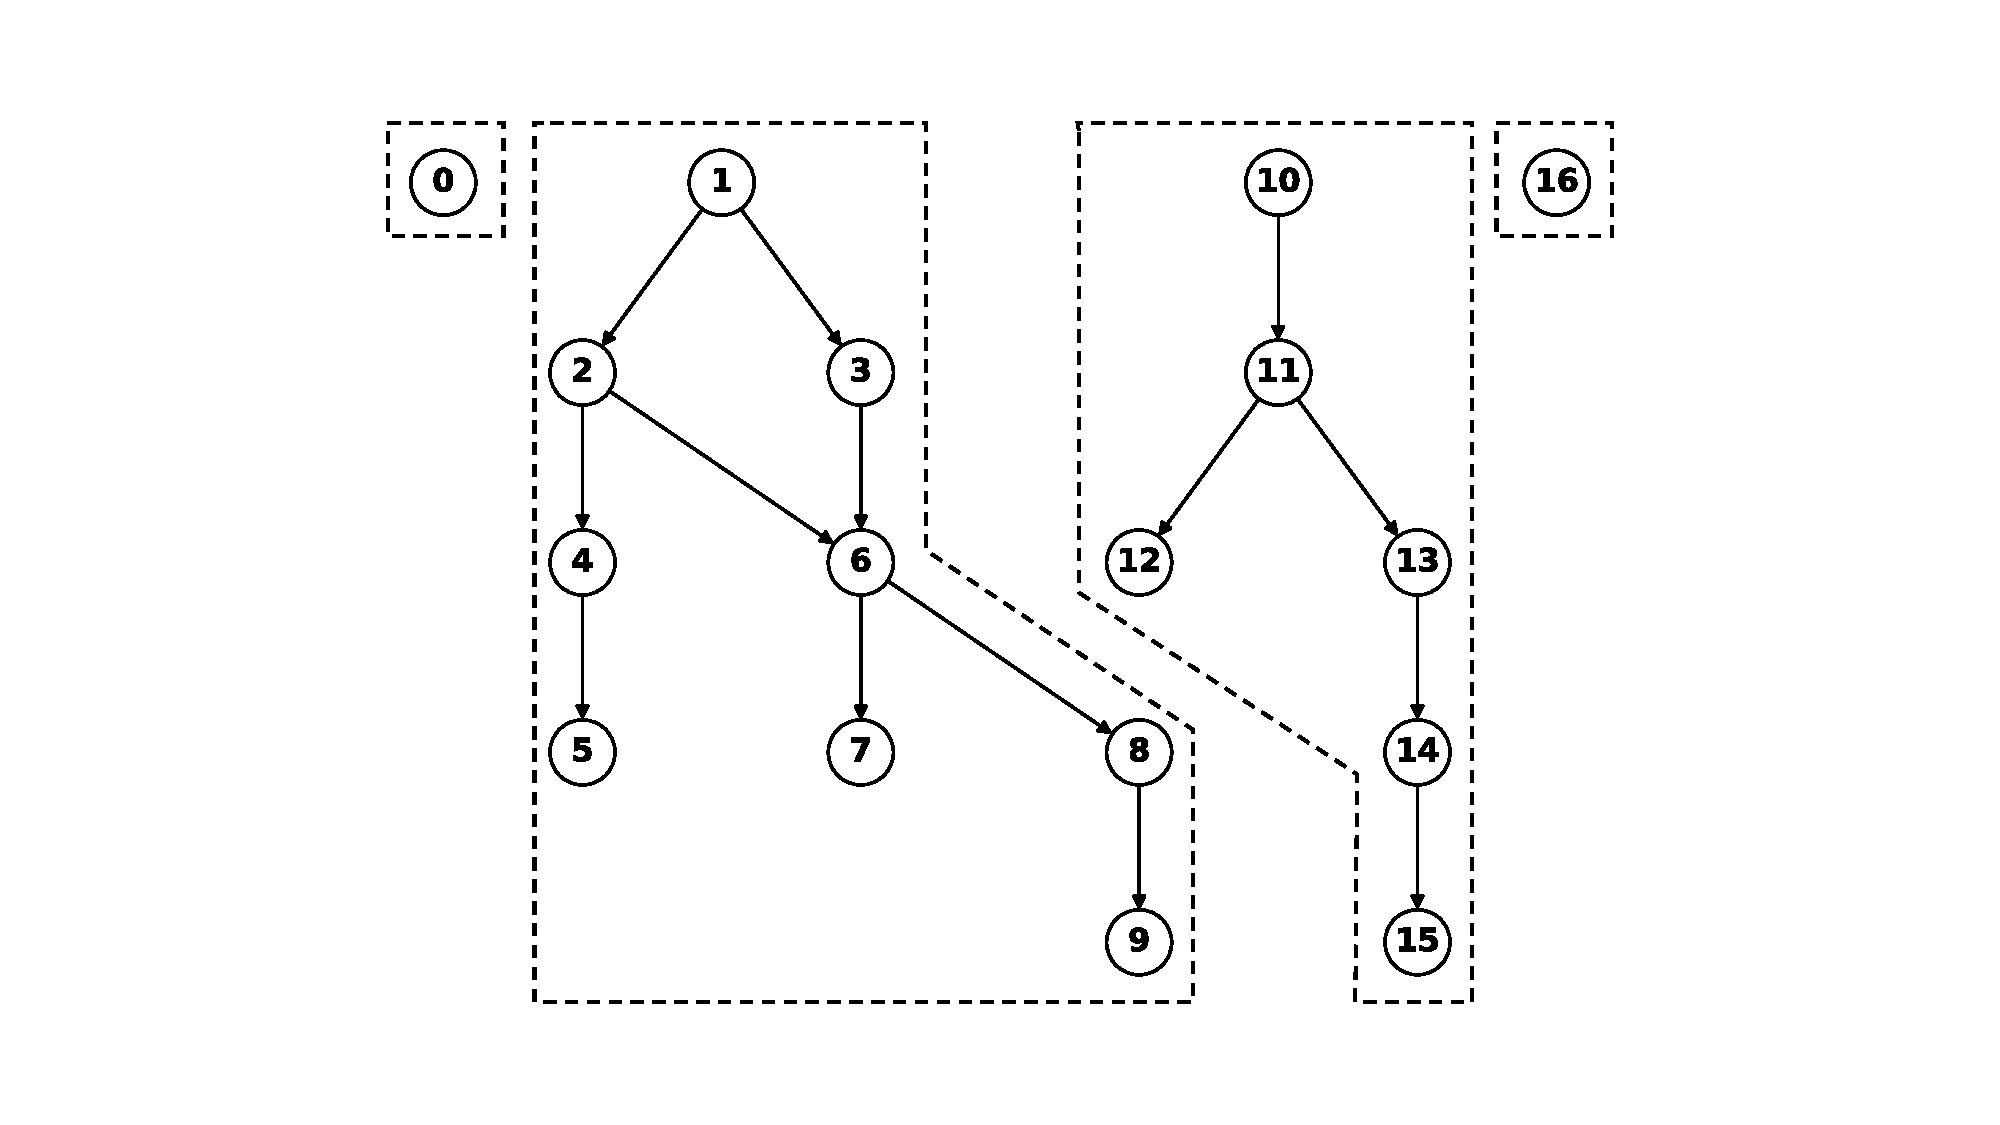
\includegraphics[scale=0.4]{fig/ifft_graph.pdf}
  \caption{IFFT application computation graph.}
  \label{fig:ifft_graph}
\end{figure}


The RL framework was also benchmarked against a collection of random directed graphs. We compare a 
PPO baseline composed of 3 MLPs stacked against an actor model with the proposed Global Graph Attention (GGA) module.
We evaluate these models on varying computation graphs complexities by increasing number of nodes in the task. 
We also tested on a larger device with 64 tiles.
In figure \ref{fig:nodes_graph}, we observe that the RL approach finds mappings for a variety of computation graphs, and GGA
improves the best schedule found for the same number of epochs. The GGA also finds improved schedule for a larger device configuration. 
In the figure \ref{fig:nodes_graph}, the epochs were limited to 50000 for both models. 
The cycle count is number of SE execution steps taken to process all nodes for a mapping, which is calculated from the simulated SE environment. 

\begin{figure}[h]
  \centering
  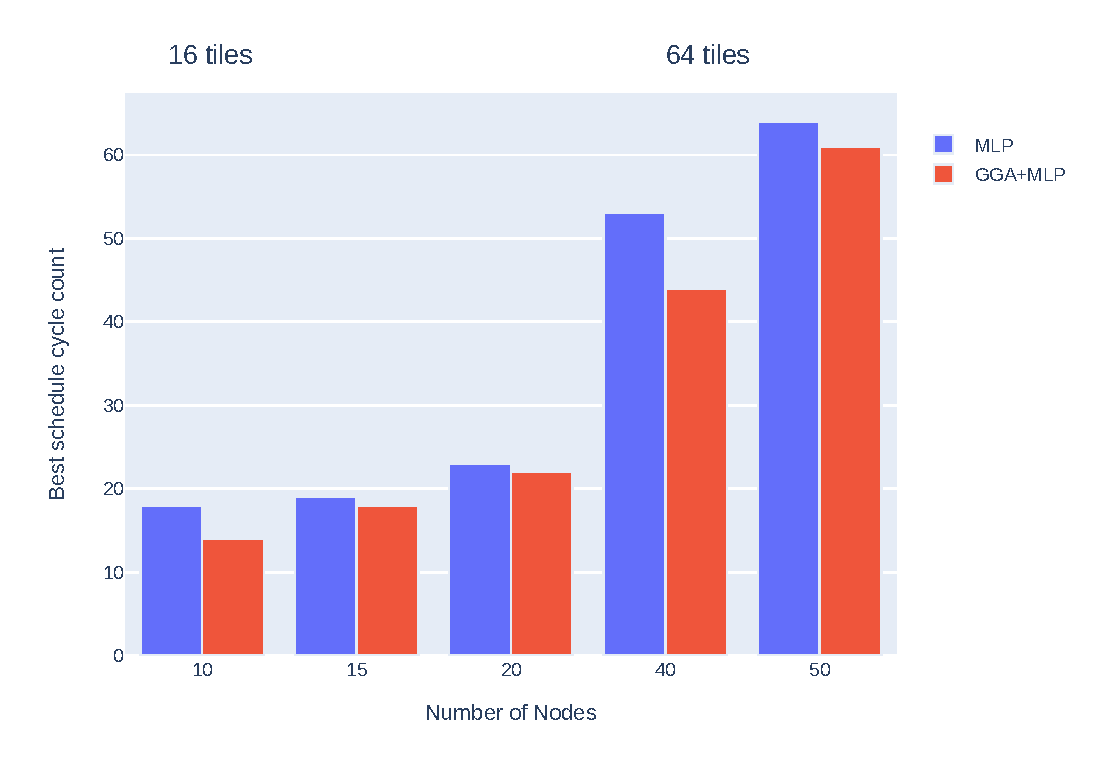
\includegraphics[width=\linewidth]{fig/nodes_graph.pdf}
  \caption{Cycle count for running all nodes in the best mapping given by RL model over 50000 epochs. 
  PPO baseline MLP model and GGA model were evaluated with computation graphs with increasing number of nodes. 
  A larger device configuration with 64 tiles was used for experiments with computation graphs with 40 and 50 nodes. }
  \label{fig:nodes_graph}
\end{figure}


\subsection{Global Graph Attention (GGA)}

In figure \ref{fig:ifft_rewards}, we see the addition of GGA module provides improved reward and sample efficiency for the IFFT application. 
The node and states changes for each iteration over all nodes in the computation graph. The GGA module provides 
a representation of the entire graph while placing each node.

\begin{figure}[h]
  \centering
  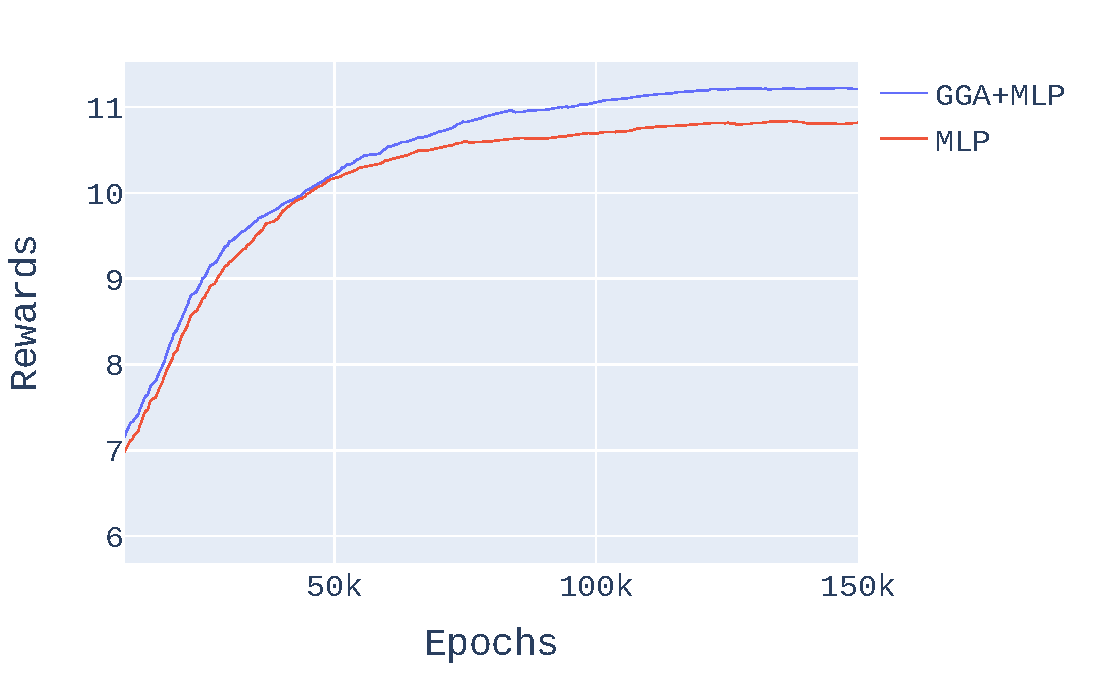
\includegraphics[width=\linewidth]{fig/plot_gnn_atten_ppo.pdf}
  \caption{Effect of using Global Graph Attention (GGA) module for mapping the IFFT application on device with 16 tiles. 
  GGA module provides better sample efficiency and higher reward after training. }
  \label{fig:ifft_rewards}
\end{figure}


\subsection{Node Iteration Order}

The iteration order that the nodes are fed to the actor model into the RL framework is important for when placing 
nodes in a sequence. In figure \ref{fig:ordered_placement}, we observe that iterating nodes in topological 
ordering results in higher reward and eases the node placement task. By placing the leaf nodes first, the model needs
to predict which tiles the predecessor nodes will be placed. This condition imposes unnecessary difficulty when training the model.

\begin{figure}[h]
  \centering
  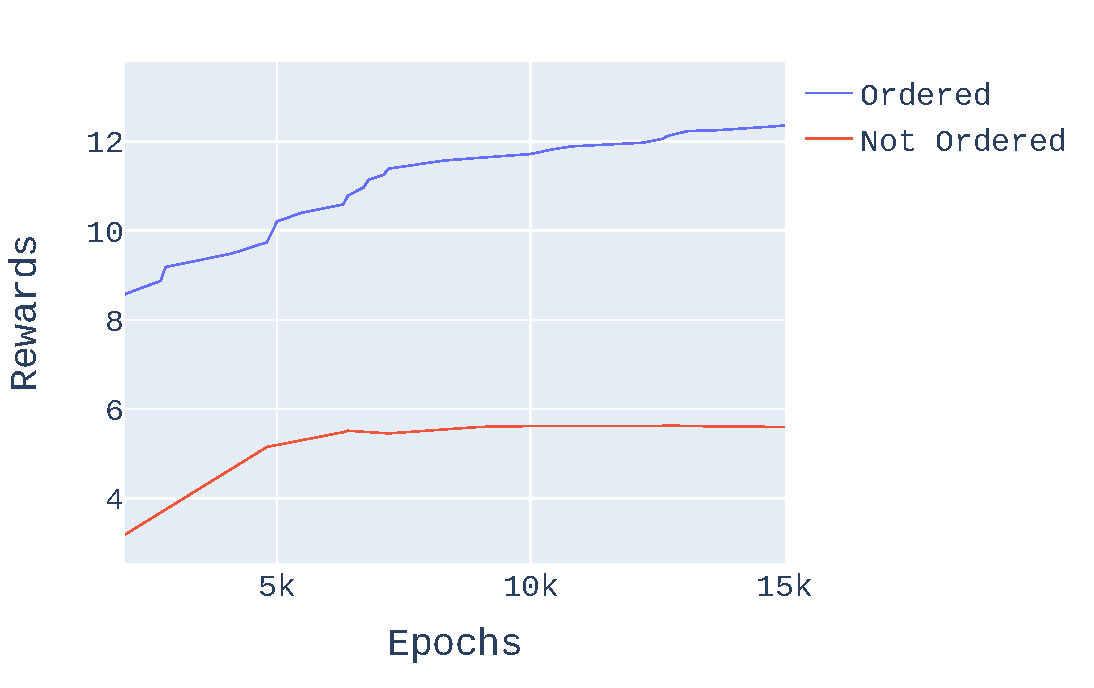
\includegraphics[width=\linewidth]{fig/plot_ordered.pdf}
  \caption{Iterating nodes in topological ordering results in higher reward and eases the placement task. 
  In blue, no order was used to place nodes. In red, nodes were iterated in topological order. 
  Task of placing 15 nodes computation graph in a device with 16 tiles.}
  \label{fig:ordered_placement}
\end{figure}


\subsection{Output Masking}

Output masking to filter invalid placements was shown effective for RL in game environments \cite{Shengyi_mask}. 
The SE instruction scheduling task has several invalid actions that adds noise to the samples and decision of the RL model. 
After placement of each node, the following nodes have less options to be placed given their data dependecy with other nodes and device constraints.
This reduces the search space as each node are being placed. 
Figure \ref{fig:mask_nomask} demonstrates that masking improves the reward and sample efficiency of the RL model.

\begin{figure}[h]
  \centering
  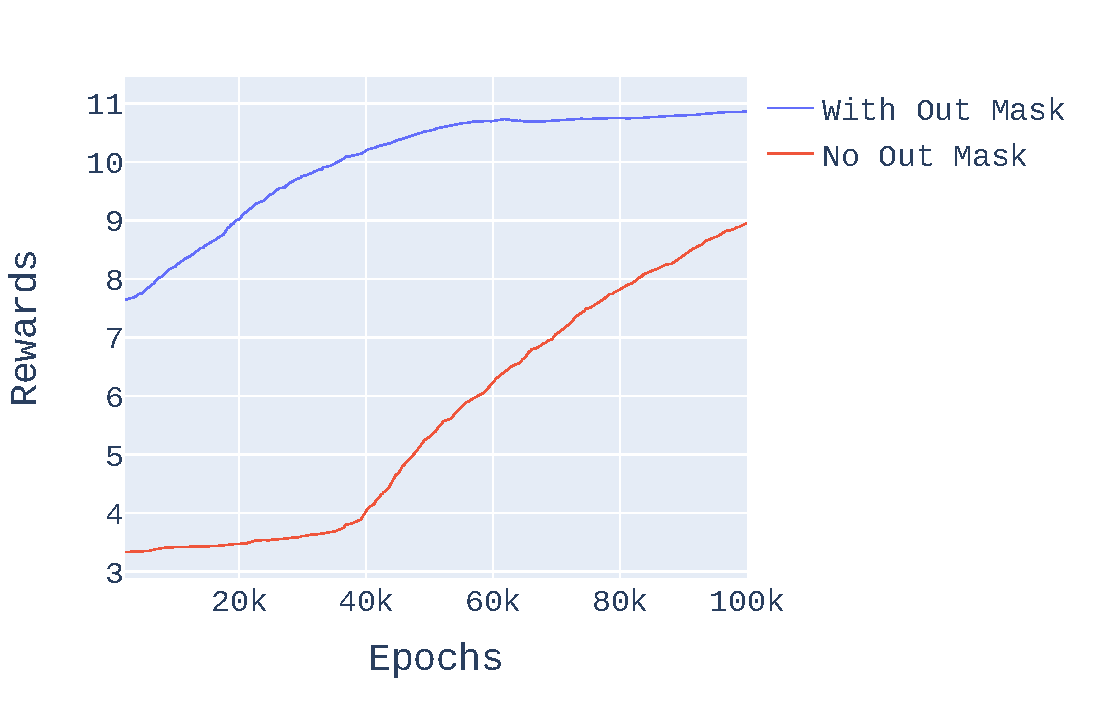
\includegraphics[width=\linewidth]{fig/ifft_masked_nomask.pdf}
  \caption{Reward comparison between node placement with output masking (blue) and without output masking (red).}
  \label{fig:mask_nomask}
\end{figure}


% sequence versus one by one


